\section{The \sm\ of Particle Physics}
\label{sec:SM}
The \sm\ of particle physics provides a consistent and precise theoretical description of known elementary particles and their interactions.
This model describes three out of four fundamental forces of nature, electromagnetic, weak and strong interactions, using a unified relativistic quantum field theory (QFT) approach with Lie group symmetries.
Gravity is not included in the \sm\ because of theoretical difficulties to formulate a consistent quantum field theory of the gravitational force. 
The gravitational coupling constant is much weaker than ones of other fundamental interactions, therefore, the gravity can be neglected for the studies presented in this thesis.

The main theoretical principles of the \sm\ were shaped by many theorists during 1960's. 
%The particle composition from the experimental point of view is completed by Higgs boson discovery at LHC experiments in July 2012, but a number of input parameters of the model are still have to be measured.

%Results of cosmological observations and few particle physics experiments reveal problems in the \sm\, therefore, this model, despite its success, cannot be a fundamental theory. 
%Nowadays, most of the modern particle physics experiments are focused on \bsm theories, that can provide answers to the existing questions in the modern physics.

%%%%%%%%%%%%%%%%%%%%%%%%%%%%%%%%%%%%%%%%%%%%%
%%%%%%%%%%%%%%%%%%%%%%%%%%%%%%%%%%%%%%%%%%%%%
%%%%%%%%%%%%%%%%%%%%%%%%%%%%%%%%%%%%%%%%%%%%%

\subsection{Particle Content}
\label{sec:ParticleComposition_SM}
A simple illustration of the particle content of the \sm\  is given in Fig.~\ref{fig:ComponentsSM}.
All fundamental particles of the \sm\ are divided into two classes distinguished by their spin quantum number: %$s_z$:

\begin{itemize}
\item Fermions are the constituents of matter with half-integer spin. Fermions with positive spin projection quantum number or helicity are called right-handed, while ones with negative helicity are called left-handed particles. 
\item Bosons mediate interactions between fermions and have integer spin. Vector bosons have spin number $\pm 1$, while scalar bosons have zero spin. 
\end{itemize}

All fermions are organized into three generations of  doublets of left-handed particles with isospin quantum number value of $I^L_3 = \pm1/2$ and singlets of right-handed particles with zero isospin.
The matter sector of the \sm\ is subdivided into two families of particles - quarks and leptons.

%Both families, quarks and leptons, have hypercharge property under $U(1)_Y$ symmetry, which is related to an electric charge as
%\begin{equation}
%	Q = I^L_3 + Y.
%\end{equation}
All fermions are subject to electroweak interactions. Beyond, quarks carry a color charge and are, therefore, also subject to strong interactions.
The first generation of quarks, $u$ and $d$, are the fermionic constituents of protons and neutrons. 

\begin{figure}[h]
{\centering
    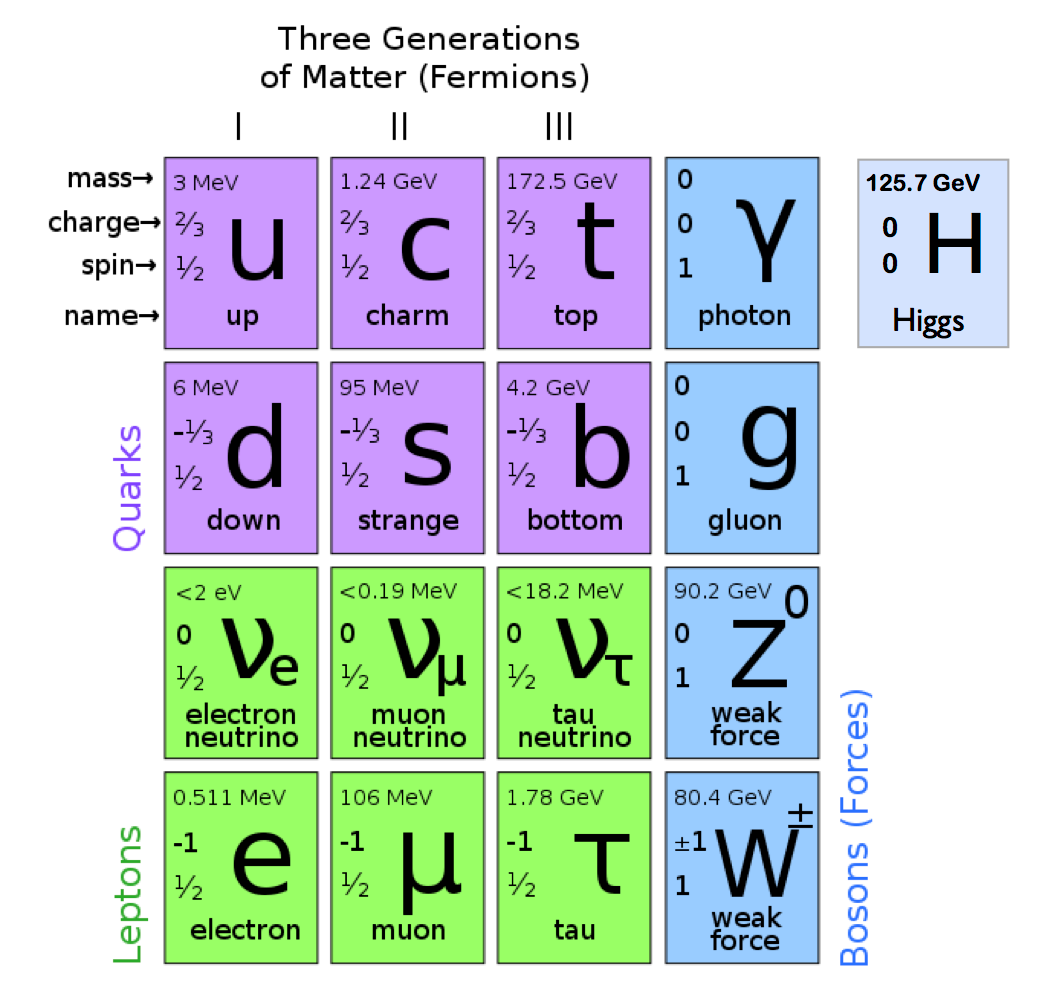
\includegraphics[width=0.55\textwidth]{graphics/Plots_Standard_Model.png}
    \caption{\sl The fundamental components of the \sm\ of particle physics.}
    \label{fig:ComponentsSM}
  }
\end{figure}
%The heaviest elementary particle in the \sm\ is the top quark.

The bosonic sector of the \sm\ consist of photon $\gamma$, $Z^0$ and $W^\pm$ bosons, gluons $g$, and scalar Higgs boson $H$.
 


\subsection{Fundamental Interactions}
\subsubsection{Electromagnetic interaction}
\label{sec:QED_SM}
%		QED
Quantum Electrodynamics (QED) is a quantum field theory, that describes an interaction between a fermionic field $\psi$ with a mass $m$ and a vector field $A_\mu$. 
The fermionic field has local $U(1)$ group invariance: %$$ group symmetry:
\begin{equation}
	\psi(x) \to e^{i\xi (x)}\psi(x).
\end{equation}
In order to preserve the local $U(1)$ symmetry, the vector field is required to be invariant under gauge transformation
\begin{equation}
A_\mu \to A_\mu (x) + \partial_\mu \xi(x).
\end{equation} 

The simplest QED Lagrangian density for a massless vector field is given by:
\begin{equation}
	\mathcal{L}_{QED}=i\bar{\psi}\gamma^\mu D_\mu \psi - \frac{1}{4}F_{\mu\nu}F^{\mu\nu},
    \label{formula:QEDlagrangian_1}
\end{equation}
where the strength tensor of the vector field is $F_{\mu\nu}=\partial_\mu A_\nu - \partial_\nu A_\mu$ and the covariant derivative is $D_\mu = \partial_\mu - ieQ A_\mu$, $e$ is a coupling constant and $Q$ is the electric charge of the fermion. 

Introduction of the covariant derivative enables fermion-photon interaction via the $-ieA_\mu\psi\gamma^\mu\bar{\psi}$ term and, moreover, it ensures the $U(1)$ symmetry in the Lagrangian density. According to the N\"other theorems, each symmetry of a Lagrangian correspond to a conserved current or charge, therefore, the $U(1)$ group symmetry of (\ref{formula:QEDlagrangian_1}) implies the conservation of the electric charge.

Scattering processes in quantum field theory can be calculated from the $S$-matrix, the time-evolution operator, which depends on the Lagrangian density of the theory. 

The fine structure constant characterizes a strength of electromagnetic interaction and it is defined in QED as $\alpha = \frac{e^2}{4\pi\epsilon_0}$. The measured value of the fine structure constant is approximately $1/137$, much smaller than 1, which allows to apply perturbation theory for $S$-matrix calculation. Each order of the perturbation series can be represented by a Feynman diagram, examples are given in Fig.~\ref{fig:FeynmanSM}. The resummation of the calculated perturbation terms is called renormalization, and it leads to the dependence of coupling constant on momentum transfer and to the corrections of particle masses. For QED the fine structure constant increases with energy and for $Z^0$ pole it has value of $\alpha(m_{Z_0}^2) \approx 1/128$.

\begin{figure}[h]
{\centering
    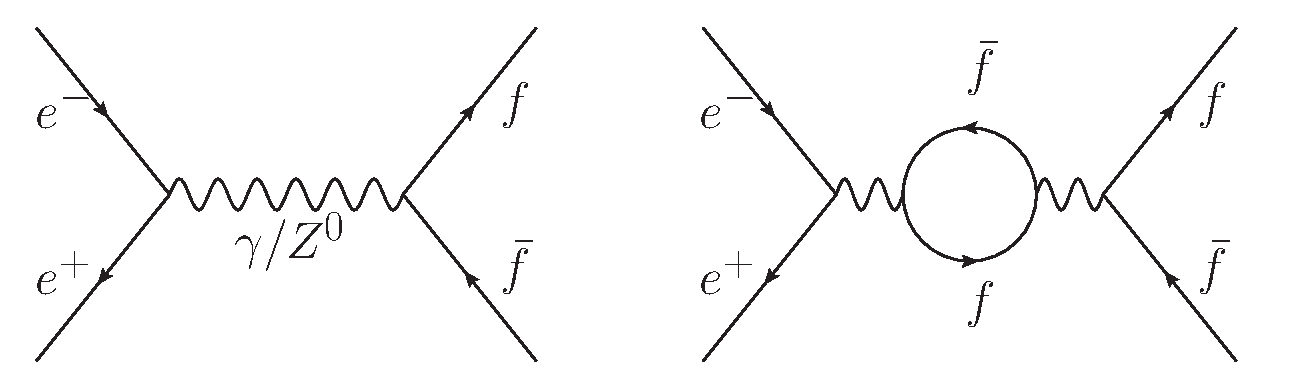
\includegraphics[width=0.55\textwidth]{graphics/FeynmanSM.eps}
    \caption{\sl Example of Feynman diagrams for $e^+e^- \to f\bar{f}$ process for Leading Order (left) and Next to Leading Order (right). }
    \label{fig:FeynmanSM}
  }
\end{figure}

QED is an accurate theory of electromagnetic interactions, that has been tested to a high precision. 
Towards the higher energies, other phenomena set in, which leads to the introduction of new forces and particles. 

%%%%%%%%%%%%%%%%%%%%%%%%%%%%%%%%%%%%%%%%%%%%%
%%%%%%%%%%%%%%%%%%%%%%%%%%%%%%%%%%%%%%%%%%%%%
%%%%%%%%%%%%%%%%%%%%%%%%%%%%%%%%%%%%%%%%%%%%%
\subsubsection{Electroweak interactions}
\label{sec:EWT_SM}
The first theory of weak interactions was developed by Fermi to describe the $\beta$ decays of unstable nuclei. The Fermi theory based on an interaction of fermionic currents without any gauge boson mediators. The Fermi coupling constant $G_F$ has a dimension of GeV$^{-2}$. This gives a strong evidence that this theory is not fundamental. The discovered weak bosons $Z^0$ and $W^\pm$ have masses far above typical energy transfer in radioactive decays of a nucleus, therefore, the Fermi theory is a low energy limit of modern Electroweak theory.

The experiments with $\beta$-decays of unstable nuclei in 1950's established maximal parity violation of weak charged currents, that involve only left-handed electrons and right-handed positrons. 

The unified theory of electroweak interaction, which was introduced by Glashow, Weinberg and Salam in 1960's, predicted the existence of weak neutral currents and the corresponding $Z^0$ boson, which can couple to right-handed particles. 
The first indications of weak neutral currents were observed at Gargamelle bubble chamber at CERN, and then, the discovery was confirmed by SPS experiments also at CERN in 1983. 

The weak interaction of the \sm\ is based on non-abelian $SU(2)_L$ symmetry group. The number of generators of a group is equal to number of gauge bosons in theory. However, taking into account the boundary condition of group unitarity, there are 3 bosons of weak force. 

The Electroweak theory operates massless $SU(2)_L$ gauge fields $W^a_\mu$ and $U(1)$ vector field $B_\mu$. The vector fields $W^a_\mu$ are initially coupled only to the left-handed fermion doublets.

The strength of the $SU(2)_L$ gauge field $W_m^a$ is defined as
\begin{equation}
	F_{mn}^a =  \partial_m W_n^a - \partial_n W_m^a + g \epsilon_{abc}W_m^b W_n^c,
    \label{formula:weakF_1}
\end{equation}
where $g$ is a coupling constant and structure constant $\epsilon_{abc}$ is the Levi-Civita tensor. The last term in (\ref{formula:weakF_1}) introduces gauge boson self-interactions, contrary to abelian QED model. 

One introduces weak mixing angle $\sin\theta_W$ relating the massless eigenstates of the weak fields and the physical mass eigenstates of the fields as:% along with the relation between massless weak eigenstate fields and physical mass eigenstate bosons:
\begin{equation}
\begin{array}{l}
W^\pm_\mu = \frac{1}{\sqrt{2}}(W^1_\mu \mp iW^2_\mu )\\
Z_\mu = W^3_\mu \cos\theta_W - B_\mu \sin\theta_W\\
A_\mu = W^3_\mu \sin\theta_W + B_\mu \cos\theta_W,
\end{array}
\label{formula:ZWafterSB_1}
\end{equation}
where $W^\pm_\mu$ and $Z_\mu$ are the physical states of the weak bosons, $A_\mu$ is the physical photon field. 
The electric coupling constant from QED is defined as 
\begin{equation}
e = g\sin\theta_w = g'\cos\theta_w,
\end{equation}
where $g$ and $g'$ are the coupling constants of weak eigenstate fields.

The Lagrangian density of mass eigenstates contains weak currents, that have a vector-axial vector (V-A) structure:
\begin{equation}
\mathcal{L}_{EW,int} = \frac{g}{2\sqrt{2}}\bar{\Psi}\gamma^\mu(1-\gamma^5)W^\pm_\mu\Psi' +\frac{g}{2\cos\theta_w} \bar{\Psi}\gamma^\mu(g_V-g_A\gamma^5)Z_\mu\Psi,
    \label{formula:weakLagrangian_1}
\end{equation}
where $g_V$ and $g_A$ are the vector and axial vector coupling constants of $Z^0$ boson to a fermionic field $\Psi$. 
As can be seen from (\ref{formula:weakLagrangian_1}), due to the mixing, the $Z^0$ boson is coupled to both, left-handed and right-handed, fermions, while the $W^\pm$ bosons are coupled only to the left-handed fermions.

The $Z^0$ and $W^\pm$ bosons acquire their masses via spontaneous symmetry breaking and the Higgs mechanism, described in Section \ref{sec:Higgs_SM}.

%%%%%%%%%%%%%%%%%%%%%%%%%%%%%%%%%%%%%%%%%%%%%
%%%%%%%%%%%%%%%%%%%%%%%%%%%%%%%%%%%%%%%%%%%%%
%%%%%%%%%%%%%%%%%%%%%%%%%%%%%%%%%%%%%%%%%%%%%

\subsubsection{Strong interaction}
\label{sec:QCD_SM}
The strong force is described by Quantum Chromodynamics (QCD), which is a relativistic quantum field theory based on $SU(3)$ symmetry.
The strong force is mediated by eight massless vector gauge bosons called gluons. 
General QCD Lagrangian density of quark fermion $q$ and gluon vector field $G^a_\mu$ is
\begin{equation}
	\mathcal{L}_{QCD}=\bar{q}(i\gamma^\mu D_\mu - M ) q - \frac{1}{4}G^a_{\mu\nu}G^{\mu\nu}_a,
    \label{formula:strongLagrangian_1}
\end{equation}
where the covariant derivative $D_\mu = \partial_\mu - i g t_a G^a_\mu$, $g_s$ is the strong coupling constant and $t_a$ are the Gell-Mann matrices being the generators of the $SU(3)$ group. The gluon field strength is
\begin{equation}
G^a_{\mu\nu}=\partial_\mu G^a_\nu - \partial_\nu G^a_\mu - g_s f_{abc}G_\mu^b G_\nu^c,
\end{equation}
where $f_{abc}$ is a structure constant tensor for $SU(3)$ group. 
Similarly to the weak interaction, QCD theory is based on a non-Abelian symmetry group and it also contains the vector boson self-interaction terms in the Lagrangian density. 

The non-Abelian quantum field with massless gauge bosons demonstrate different the asymptotic behavior of coupling constant: the strong fine-structure constant $\alpha_{s0} = g_s^2/(4\pi)$ depends on momentum transfer squared $Q^2$ as 
\begin{equation}
\alpha_{s}(Q^2) \propto ln^{-1}(Q^2),
\end{equation}
which means, that the strength of QCD interaction is decreasing for high energy processes. This effect of QCD is called asymptotic freedom. On the other hand, when momentum transfer is small, the $\alpha_{s}$ becomes large. Theoretical prediction of $\alpha_s(Q)$ and the results of $\alpha_s$ measurements are shown in Fig.~\ref{fig:alpha_s}. This behavior of $\alpha_s(Q)$ leads to the effect of color confinement, when quarks and gluons form colorless objects called hadrons. For low energy processes, the perturbation theory cannot be applied because of the strong QCD coupling. Therefore, the low-energy QCD processes and the color confinement effects are analyzed using Lattice QCD methods. 
\begin{figure}[h]
{\centering
    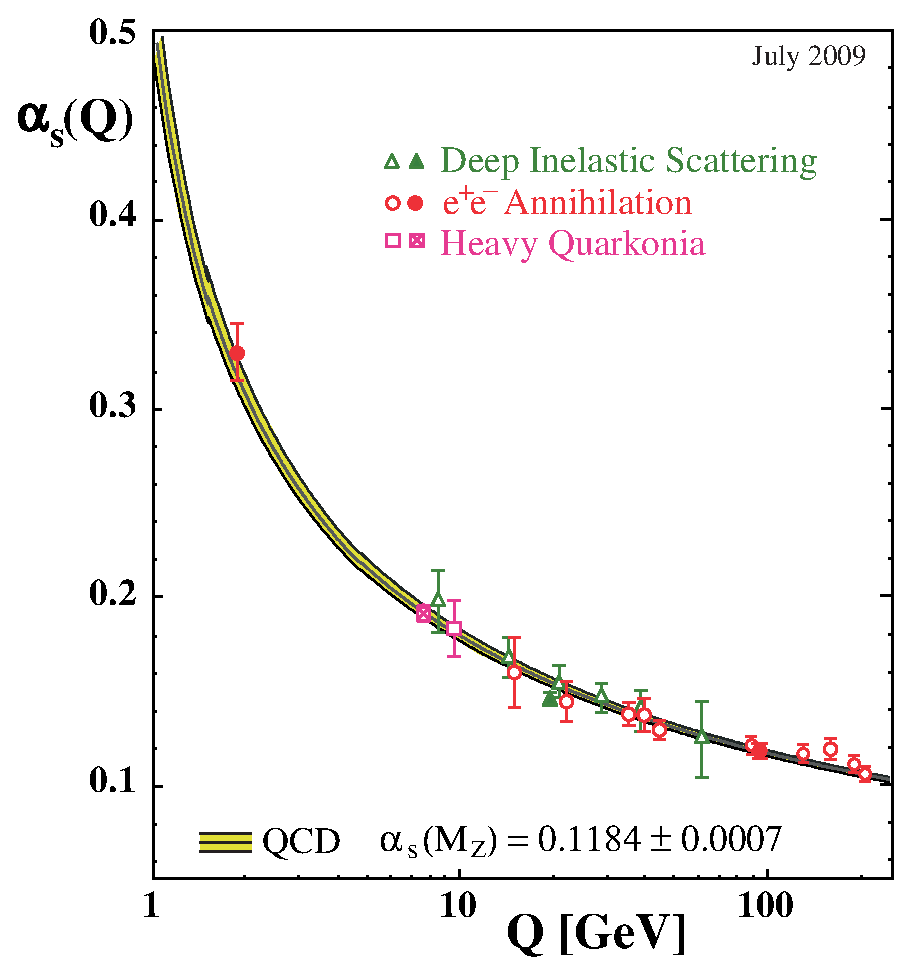
\includegraphics[width=0.45\textwidth]{graphics/asq-2009.eps}
    \caption{\sl Summary of measurements of $\alpha_s$ as a function of the energy scale $Q$.\cite{bib:alpha_s}}
    \label{fig:alpha_s}
  }
\end{figure}

%So far, the only quark, that does not have a hadronic final state is the top quark. Because of its high mass, it decays via weak interaction before a formation of any hadronic states. 

%%%%%%%%%%%%%%%%%%%%%%%%%%%%%%%%%%%%%%%%%%%%%
%%%%%%%%%%%%%%%%%%%%%%%%%%%%%%%%%%%%%%%%%%%%%
%%%%%%%%%%%%%%%%%%%%%%%%%%%%%%%%%%%%%%%%%%%%%

\subsection{The Higgs mechanism}
\label{sec:Higgs_SM}
% Higgs is the only elementary scalar in the \sm
%Why?
%Goldstone bosons???
Classical mass terms for quantum fields without symmetry breaking mechanism cause the following problems:
\begin{itemize}
	\item Term $m_A A_\mu A^\mu$ for a vector field $A_\mu$ introduce an ultraviolet divergence in the massive vector field propagator;
	\item Terms like $m_\psi\psi_L \psi_R$ are not gauge-invariant, since right-handed and left-handed fermions have different set of quantum numbers in the \sm.
\end{itemize}
The mechanism of spontaneous symmetry breaking or the Higgs mechanism is an essential part of fundamental physics. 
It allows to include the weak vector boson masses in a renormalizable way and to  preserve the gauge invariance of fermion mass terms in the Lagrangian density of the \sm. 

%DOUBLET
The spontaneous symmetry breaking mechanism starts from a complex scalar field doublet $\phi$ , which has initially four degrees of freedom. 
The Lagrangian density, related to the scalar field, which is coupled to $SU(2)$ gauge field $W_\mu$ and $U(1)$ vector field $B_\mu$, has the following terms: 
%The higgs symmetry???
\begin{equation}
	\mathcal{L}_{H} = \frac{1}{2}(D_\mu\phi)^2 - V(\phi),
    \label{formula:scalarLagrangian_1}
\end{equation}
where covariant derivative $D_\mu = \partial_\mu - i g \tau_a W^a_\mu - ig'/2 B_\mu$ and the matrices $\tau_a$ are the $SU(2)$ group generators. This Lagrangian density has a $SU(2) U(1)$ symmetry.
The form of the scalar field potential $V(\phi)$ is in general case 
\begin{equation}
    V(\phi) = -\frac{1}{2}\mu^2|\phi|^2 +  \frac{1}{4} \lambda |\phi|^4.
\end{equation}
If the parameter $\mu^2 > 0$, the scalar field $\phi$ will acquire a nonzero vacuum expectation value  %and the $SU(2)$ local symmetry will be broken:
\begin{equation}
\phi_0 = \frac{1}{\sqrt{2}}
\begin{pmatrix}
0\\v
\end{pmatrix} \text{ and } v = \sqrt{\frac{\mu^2}{\lambda}}, 
\end{equation}
which breaks local $SU(2)$ symmetry of the Lagrangian density. 

According to the Goldstone theorem, number of broken group generators correspond to the number of massless scalar particles called Goldstone bosons. 
In the \sm\ case, the broken $SU(2)$ symmetry produces three Goldstone bosons and one Higgs boson $H$, which has a leftover degree of freedom from the initial scalar doublet $\phi$.
The three Goldstone bosons are absorbed as longitudinal degrees of freedom by vector fields $W^a_\mu$, thus giving mass to the weak bosons.

The relevant terms after symmetry breaking from (\ref{formula:scalarLagrangian_1}) are
\begin{equation}
	\Delta \mathcal{L}_{H} = \frac{1}{2} \frac{v^2}{4}[g^2 (W^1_\mu)^2 + g^2 (W^2_\mu)^2 + (-g W^3_\mu + g' B_\mu)^2].
\end{equation}
The electroweak fields acquire physical states (\ref{formula:ZWafterSB_1}) with masses
\begin{equation}
\begin{array}{l}
m_W^\pm = g\frac{v}{2},\\
m_Z^0 = \sqrt{g^2 + g'^2}\frac{v}{2},\\
m_A = 0,
\end{array}
\label{formula:ZWmassafterSB_1}
\end{equation}
and the Higgs boson mass is
\begin{equation}
m_H = \sqrt{2\lambda}v.
\end{equation}

With postulated quantum numbers of the Higgs field, one writes the gauge-invariant mass terms for a fermion $\psi$ as 
\begin{equation}
	\Delta \mathcal{L}_\psi = -\lambda_\psi \Psi_L \phi \psi_R,
\end{equation}
where dimensionless parameter $\lambda_\psi$ is a Higgs coupling to the fermion field, $\Psi_L$ is the left-handed $SU(2)$ doublet, and $\psi_R$ is the right-handed $SU(2)$ singlet. Thus, this expression has zero sum of the hypercharge $Y$, and it can be extended to all lepton particles of the \sm. The mass terms for the quark sector are more complicated, because of involvement of quark mixing, but the expression for fermion mass is universal
\begin{equation}
	m_\psi = \frac{1}{\sqrt{2}} \lambda_\psi v.
    \label{formula:fermionMass_1}
\end{equation}
% Higgs - top relation

The discovery of the Higgs scalar by LHC collaborations (see Fig.~\ref{fig:diphoton}) added the last missing piece to the \sm, and experimentally proved the principles of the mechanism of spontaneous symmetry breaking.

The expressions \ref{formula:ZWmassafterSB_1} and \ref{formula:fermionMass_1} suggest a simple linear relation between Higgs boson couplings and masses of corresponding particles. The results of the LHC experiments confirm this prediction within experimental uncertainties, as shown in Fig~\ref{fig:higgs_masses}.


\begin{figure}
\centering
\begin{subfigure}{0.5\textwidth}
\centering
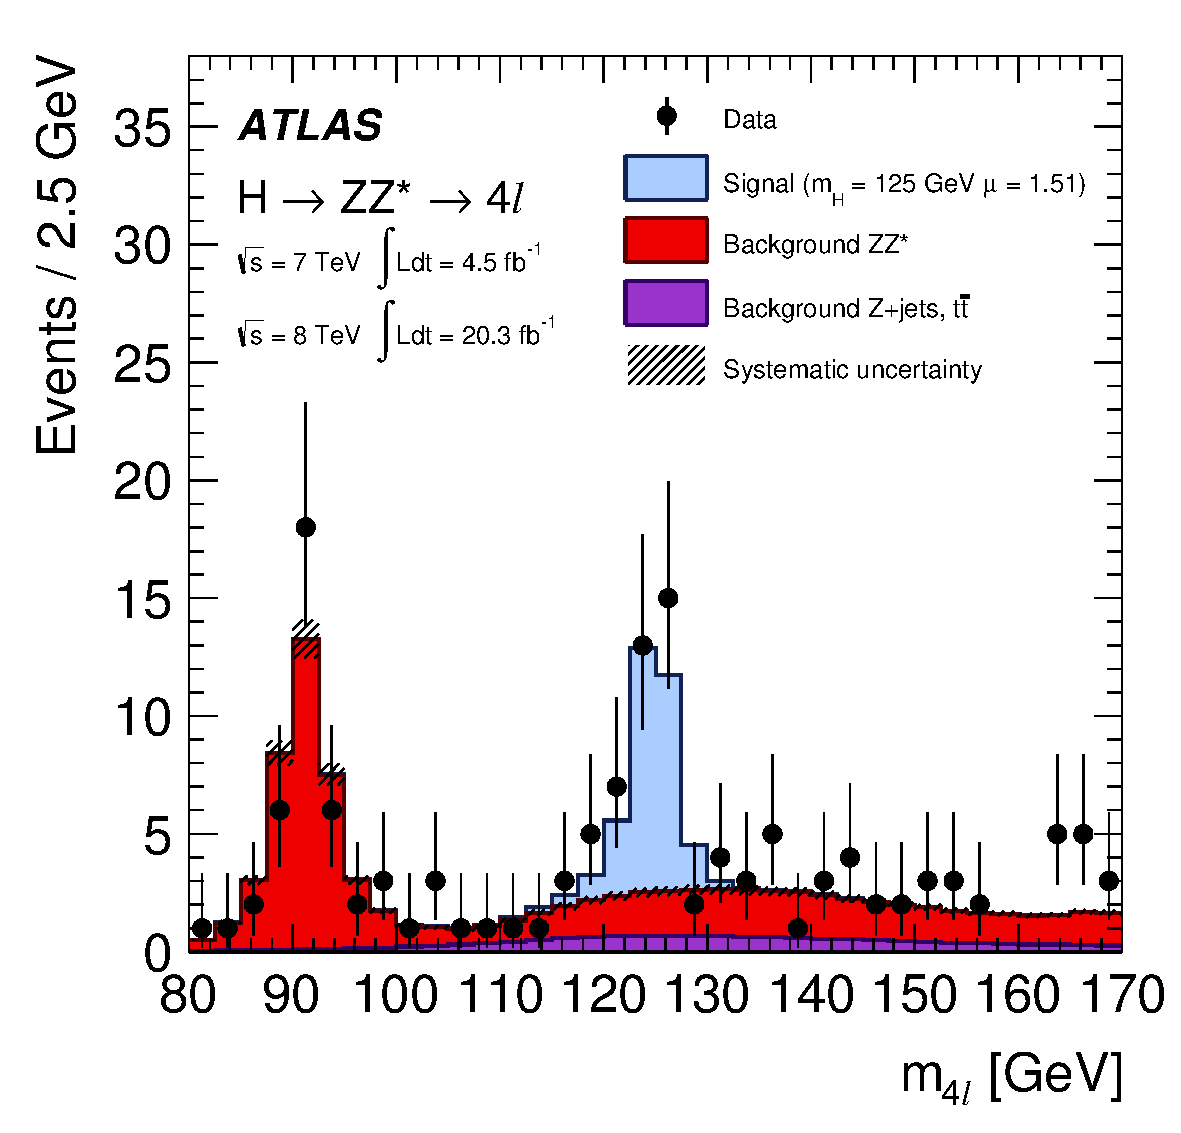
\includegraphics[width=.90\linewidth]{graphics/m4l_80_170_allYear_125.pdf}

\end{subfigure}% 
\begin{subfigure}{0.5\textwidth}
\centering
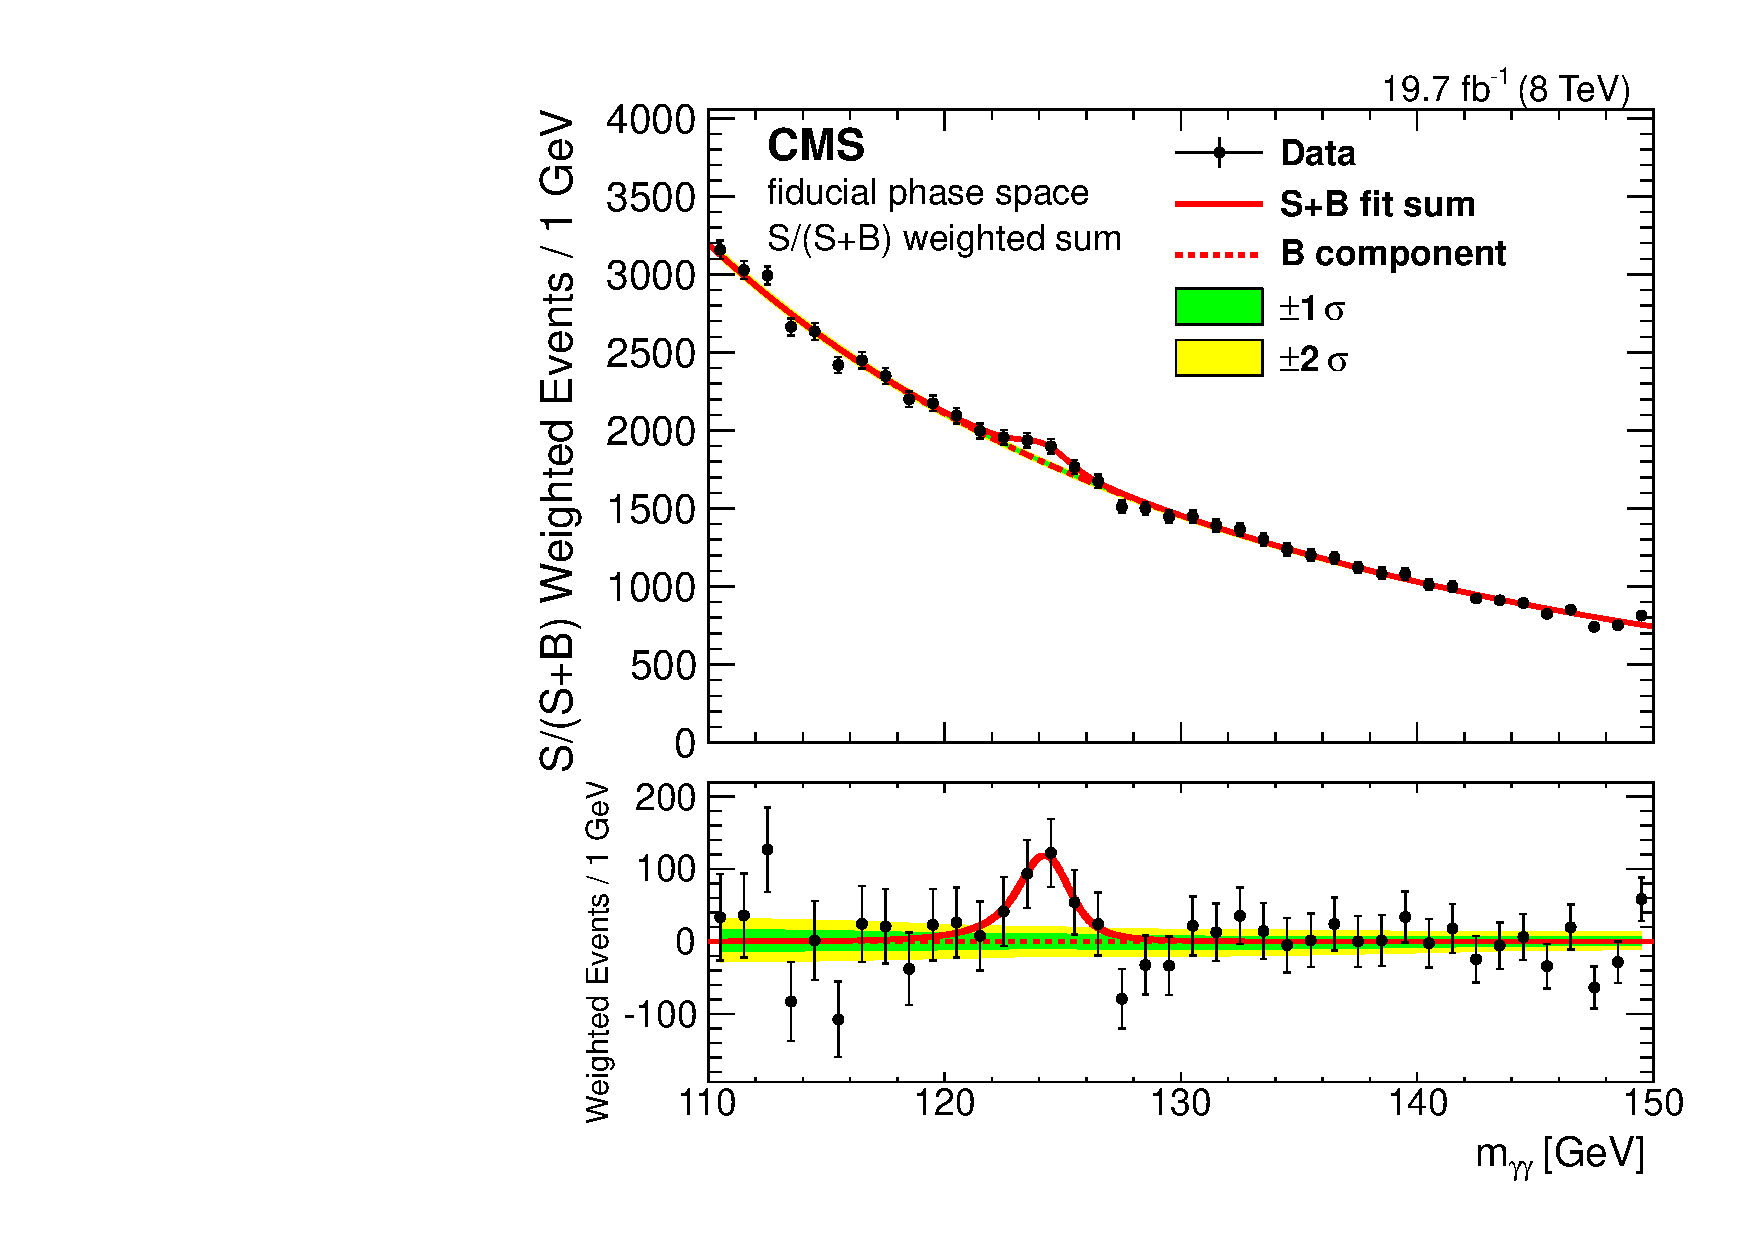
\includegraphics[width=.90\linewidth]{graphics/CMS-HIG-14-016_Figure_003.pdf}

\end{subfigure}
    \caption{\sl The Higgs boson signal in $Z^0Z^0$ channel by ATLAS (left) \cite{bib:HiggsAtlas2} and Higgs boson signal in diphoton invariant mass distribution by CMS experiment (right) \cite{bib:HiggsCms2}.}
    \label{fig:diphoton}
\end{figure}

\begin{figure}
{\centering
    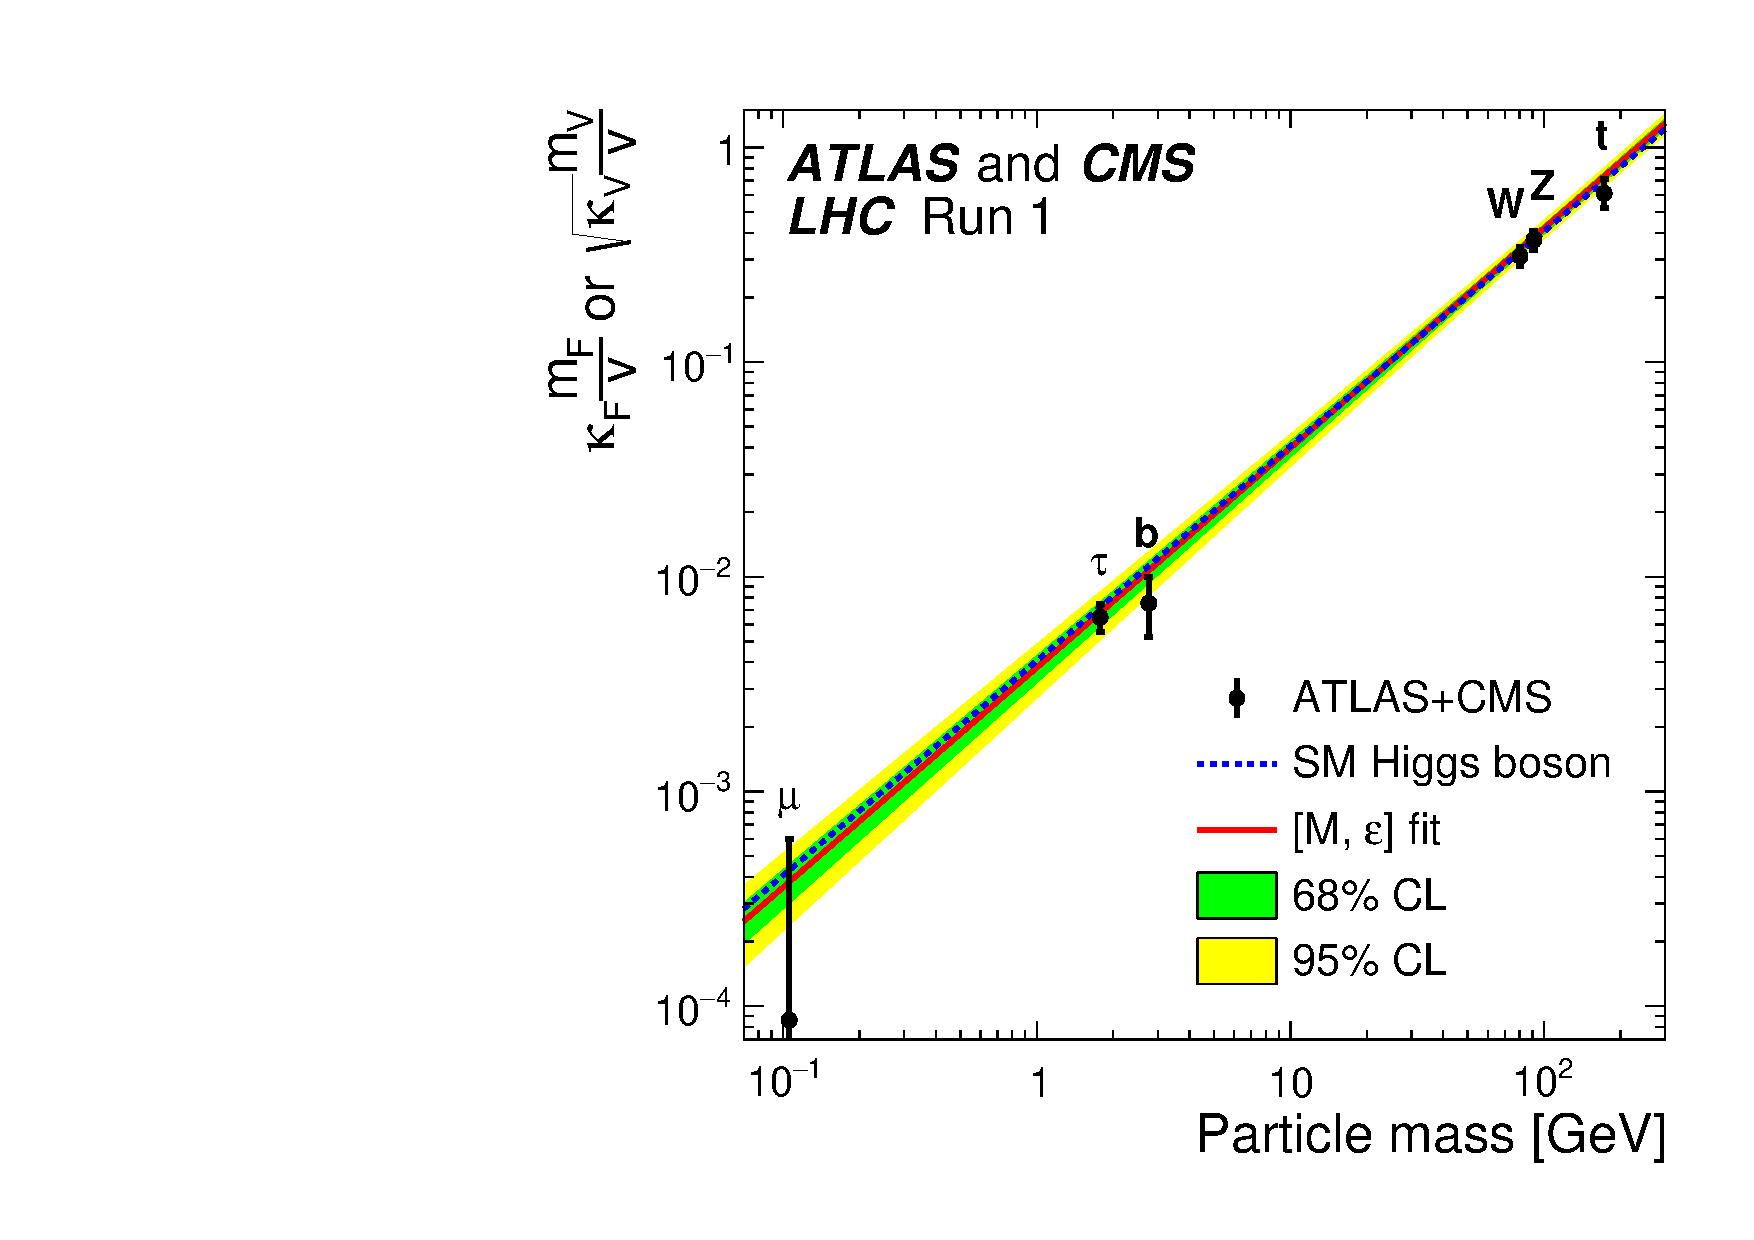
\includegraphics[width=0.45\textwidth]{graphics/Meps_lhc.pdf}
    \caption{\sl Demonstration of the linear dependence of particle masses on Higgs boson couplings by LHC experiments. \cite{bib:HiggsLhc2}}
    \label{fig:higgs_masses}
  }
\end{figure}

\subsection{The \sm\ tests and open questions in particle physics}
\label{sec:Problems_SM}
The \sm\ results from the synergy between theoretical ideas and experimental results. After finalization of the \sm\ framework, this model was able to predict many phenomena of particle physics, like the existence of weak neutral currents, top quark and Higgs boson.
The \sm\ has been tested to a high precision at the machines like HERA, SLC, LEP, TeVatron and the LHC. A summary of electroweak precision measurements compared to a \sm\ electroweak fit values is shown in Fig.~\ref{fig:SM3deviations}. The \sm\ fit demonstrates, that there are no deviation greater than 2.5~$\sigma$. 

\begin{figure}[ht]
\centering
  \includegraphics[width=0.46\textwidth]%
                  {graphics/2014_07_16_PullPlotTwoBarsTwoTheos_logo.eps}
  \caption{Deviations of the electroweak precision
observables in the Standard Model~\cite{bib:AfbSMFit}. }
  \label{fig:SM3deviations}
\end{figure}
%The muon g-2 experiments can measure muon  
%The \sm\ prediction of the $\mathcal{CP}$ violation has been confirmed by the B-meson experiments. 
The experiments, that explore rare $B$-meson decays, like BaBar, Belle or LHCb, show a good agreement with the \sm\ predictions. 
Nevertheless, some experiments in particle physics as well as a few cosmological observations have tensions with the \sm\ predictions.
The shortcomings of the \sm\ are summarized as following:
\begin{itemize}
%Gravity
\item The \sm\ provide precise and consistent explanation of interactions between three out of four fundamental forces, the gravitational force is not included. The integration of the gravity into the \sm\ framework is unsuccessful, because of non-renormalizablity of tensor quantum fields. Knowledge of quantum gravity is important for cosmology of early Universe and for physics of extremely massive astrophysical objects, like black holes.
%Higgs mass fine-tuning
\item Quantum corrections to the Higgs boson mass are large comparing to the mass of Higgs boson itself, which resembles a \textit{fine-tuning problem} of the \sm. This can be avoided if there are new massive bosons, that can stabilize the Higgs mass corrections.
\item There is no explanation of the reason behind the spontaneous symmetry breaking mechanism in the \sm\ framework. 

% mass hierarchy 
\item The particle masses in the \sm\ are proportional to the Higgs coupling constants, which are input parameters of the theory. Thus, the \sm\ do not provide any explanation of 6 orders of magnitude difference between well measured electron mass and top quark mass. This fact is known as a \textit{mass hierarchy problem}.

\item The sources of the charge-parity ($CP$) asymmetry, provided by the quark mixing matrix in the \sm, are too small to explain the \textit{matter-antimatter asymmetry} of the Universe.
\item Anomalous rotation of galaxies suggests an existence of large amount of \textit{dark matter} - massive particles, that do not interact with the electromagnetic field. The \sm\ neutrinos are too light to explain this observation, therefore, the \sm\ has no candidate particle for dark matter. 
%Afb bbbar
%g-2

\end{itemize}



Many \bsm\ theories propose elegant solutions to the shortcomings of the \sm\ mentioned above, and many experiments are looking for their evidences. 
This thesis proposes new tests of the \sm\ using the ILC project, which will provide new evidences of New Physics with a discrimination power between different \bsm\ theories.
%At the same time, there is a lack of knowledge about many input parameters of the \sm, and high precision measurements can give further hints for New Physics.

%Dark matter there are many theoretical solutions that resemble gravity modifications

